\documentclass[11pt,a4paper,oneside]{article}
% input the config file
\usepackage[a4paper,margin=0.5in]{geometry}
\usepackage[separate-uncertainty=true,range-phrase=--]{siunitx}
\usepackage[utf8]{inputenc}
\usepackage[T1]{fontenc}
\usepackage{mathtools}
\usepackage{amsfonts}
\usepackage{amsthm}
\usepackage{booktabs}
\usepackage{thmtools}
\usepackage{amssymb}
\usepackage{graphicx}
\usepackage{enumitem}
\usepackage{tabularx} 
\usepackage[sfdefault]{roboto}
\usepackage[bibstyle=numeric,citestyle=alphabetic,natbib=false,backend=biber,sorting=ynt,sortcites=true,autocite=plain,hyperref=true,backref=true,maxbibnames=15,minbibnames=10,maxnames=15,minnames=10]{biblatex}
\usepackage{csquotes}
\usepackage{fancyhdr}
\usepackage{titlesec}
\usepackage{lipsum}
\usepackage{multicol}
\usepackage{flafter}
\usepackage{wrapfig}
\usepackage[usenames,dvipsnames]{xcolor}
\usepackage{pagecolor}
\usepackage{tcolorbox}
\usepackage[pdftex,hyperfootnotes=false,pdfpagelabels]{hyperref}
\usepackage[capitalise,noabbrev]{cleveref}
% no indentation for paragraphs, instead add more vertical spacing
\usepackage[skip=1ex,indent=0em]{parskip}

% make links/urls in bold
% https://tex.stackexchange.com/questions/47468/how-to-make-url-bold
\def\UrlFont{\bfseries}
% https://tex.stackexchange.com/questions/351650/make-all-href-text-bold
\LetLtxMacro\oldhref\href
\RenewDocumentCommand{\href}{o m m}{%
  \IfValueTF{#1}
    {\oldhref[#1]{#2}{\bfseries #3}}
    {\oldhref{#2}{\bfseries #3}}%
}
\addbibresource{bibliography.bib}

\titleformat{name=\section}{\huge\bfseries\sffamily\color{BlueViolet}}{\thesection}{.5em}{}
\renewcommand{\headrulewidth}{0pt}

% https://tex.stackexchange.com/a/17101/11281
% for logos in the same line as text in title page
\newcommand{\vcenteredinclude}[1]{\begingroup
  \setbox0=\hbox{\includegraphics[keepaspectratio,height=4ex]{#1}}%
\parbox{\wd0}{\box0}\endgroup}

% For section authors
\newcommand{\sectionauthor}[1]{\begingroup
{\color{Blue}\textbf{\large #1\\}}\rule{\textwidth}{0.4pt}\endgroup}

% Make submitter names bold in references
% The bibliography entry must include another field for this
% https://tex.stackexchange.com/a/304968/11281
\renewcommand*{\mkbibnamegiven}[1]{%
  \ifitemannotation{highlight}
    {\textbf{#1}}
    {#1}}

\renewcommand*{\mkbibnamefamily}[1]{%
  \ifitemannotation{highlight}
    {\textbf{#1}}
    {#1}}


%\definecolor{ocnspagecolor}{RGB}{255, 241, 213}
\definecolor{ocnspagecolor}{RGB}{255, 250, 241}


% document begins
\begin{document}

\pagestyle{plain}
\newgeometry{top=0mm,bottom=0mm,left=0mm,right=0mm}
\begin{titlepage}
  \quad{}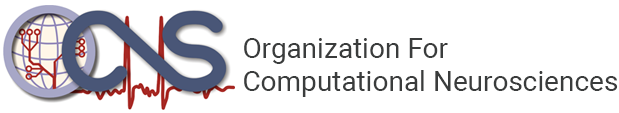
\includegraphics[width=0.8\textwidth,keepaspectratio]{./images/ocns-logo}
  \begin{tcolorbox}[colback=gray, colframe=black, width=\textwidth, boxrule=0.5mm, leftrule=0mm, rightrule=0mm,sharp corners=all]
  \vspace{1ex}
  \textbf{\textcolor{white}{Member Newsletter\quad{}|\quad{}October 2024\quad{}|\quad{}Volume 8 No 2}}
  \vspace{1ex}
  \end{tcolorbox}
  \topskip0pt
  \vspace{-1.35ex}
  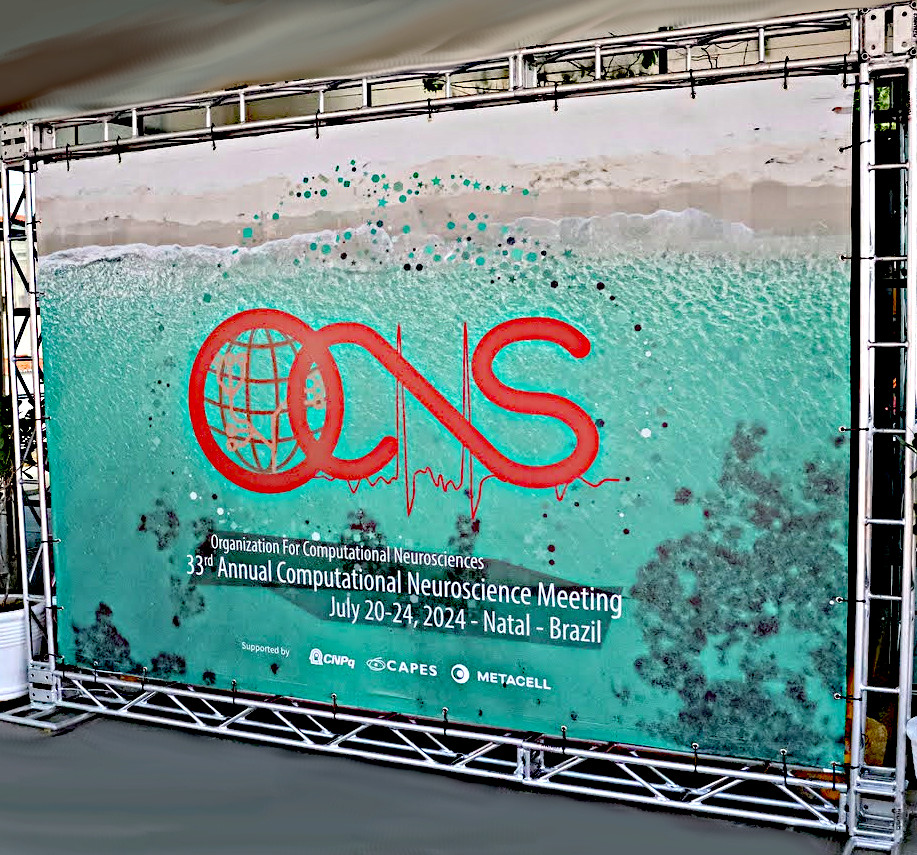
\includegraphics[width=\linewidth,keepaspectratio]{./images/ocns-newsletter-cover}
  \vspace{4ex}

  \vspace{1ex}
  \begin{center}
    \href{https://mastodon.social/@OCNS}{\vcenteredinclude{./images/Mastodon_Logotype_(Simple).svg}}~
    \href{https://twitter.com/cnsorg}{\vcenteredinclude{./images/X-logo}}~
    \href{https://www.facebook.com/CNSorg/}{\vcenteredinclude{./images/Facebook_icon_2013.svg}}~
    \textbf{\Large @CNSOrg}
    \hspace{1.2cm}\href{https://www.instagram.com/cns_ocns/}{\vcenteredinclude{./images/cropped-black-instagram-logo}}~
    \textbf{\Large @cns\_ocns}
    \hspace{1.2cm}\href{https://www.youtube.com/@ocns9820}{\vcenteredinclude{./images/youtube-logo}}~
    \textbf{\Large @ocns9820}
    \hspace{1.2cm}\href{https://www.linkedin.com/company/organization-for-computational-neurosciences/}{\vcenteredinclude{./images/LinkendIn}}~
    \textbf{\Large @OCNS}\vspace*{\fill}
  \end{center}
\end{titlepage}

\restoregeometry

\clearpage

\pagestyle{fancy}
\fancyhead{}
\fancyfoot{}
\fancyfoot[L]{Volume 8 No 2}
\fancyfoot[C]{OCNS Newsletter}
\fancyfoot[R]{Page \thepage}

\clearpage
\pagecolor{ocnspagecolor}
\section*{Message from the President}%
\sectionauthor{Thomas Nowotny, Professor of Informatics, University of Sussex, UK}
\begin{wrapfigure}{l}{0.2\textwidth}
  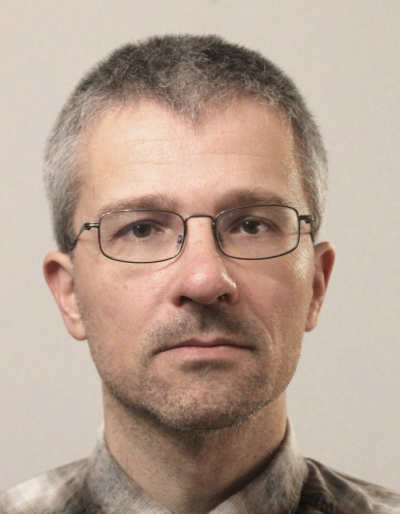
\includegraphics[width=0.2\textwidth]{images/Thomas}
\end{wrapfigure}

\lipsum[1-3]

\centerline{\rule{0.5\textwidth}{0.4pt}}
\vspace{1ex}
\begin{center}
\begin{tcolorbox}[colback=CornflowerBlue, colframe=black, width=0.9\textwidth, boxrule=0.1mm]
See pictures from CNS*2024 Natal here: \url{https://www.cnsorg.org/cns-2024-photo-album}.
\end{tcolorbox}
\end{center}
\centerline{\rule{0.5\textwidth}{0.4pt}}
\vspace{1ex}

\section*{CNS*2024 Natal: From the Program Chair}%
\sectionauthor{Program Chair:\ Julie Haas, Lehigh University, USA}
\begin{wrapfigure}{l}{0.2\textwidth}
  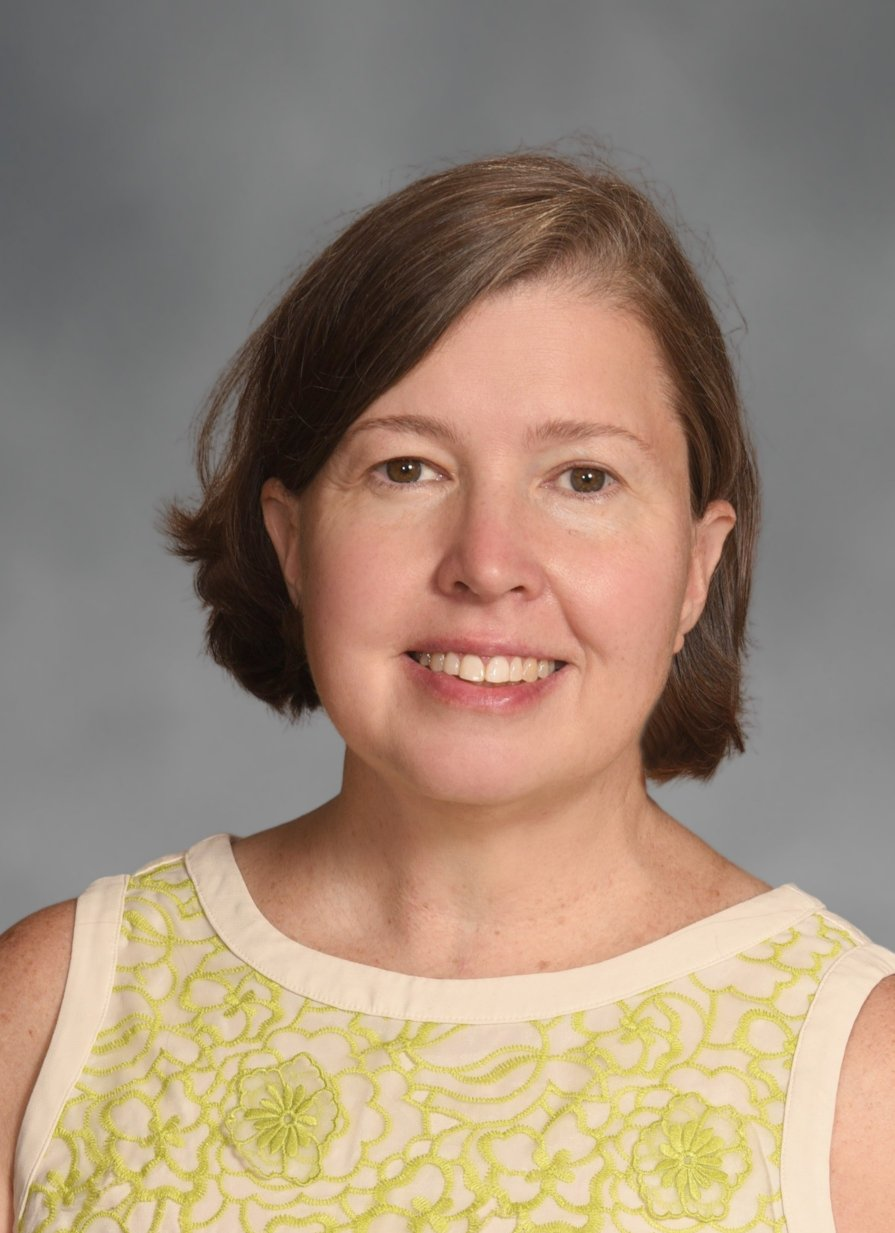
\includegraphics[width=0.2\textwidth]{images/Haas}
\end{wrapfigure}

Many thanks to Axel Hutt (Deputy Chair), Sang Wan Lee, Ian Stevenson and Nassi Papoutsi for their service on the Program Committee, and extend a warm welcome to Andre Peterson, Masanori Shimono, Yunliang Zang and Arezoo Alizadeh.
We're currently working on selecting keynotes for CNS*2025 Florence, and look forward to a robust round of abstract reviewing in spring.

\clearpage
\section*{CNS*2024 Natal: in charts}%
\vspace{-4ex}
\sectionauthor{}
\begin{figure}[ht]
  \centering
  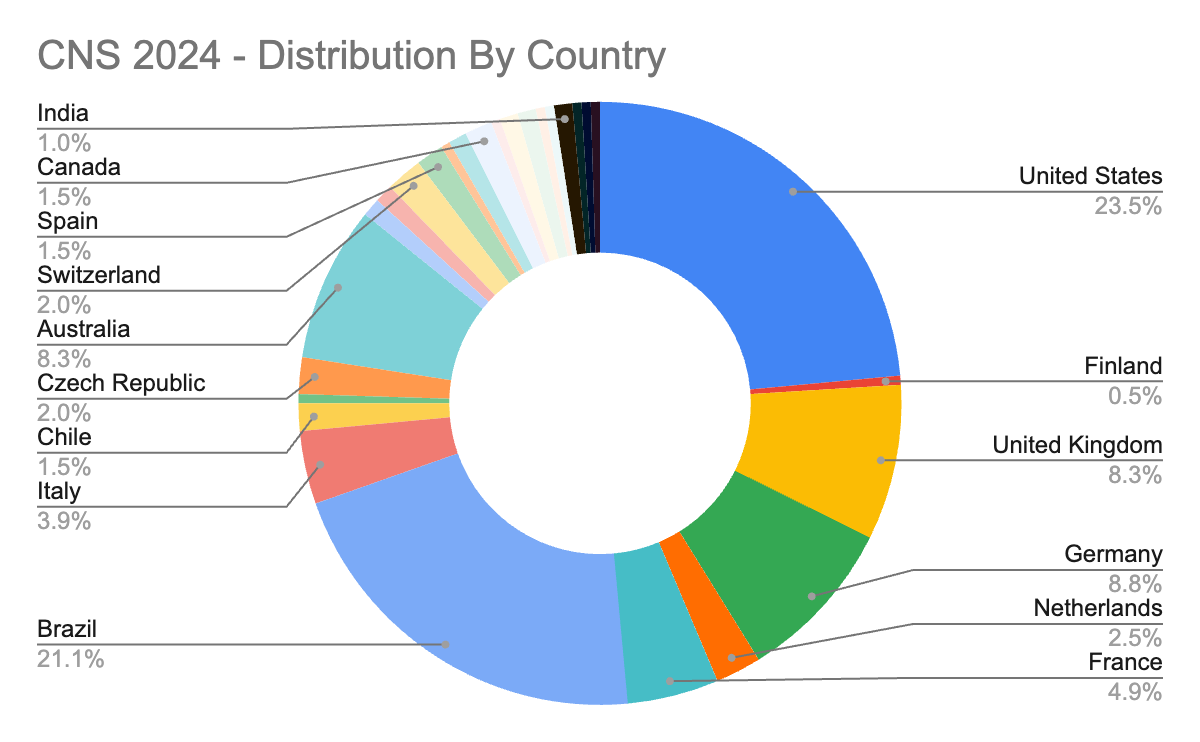
\includegraphics[width=0.9\textwidth]{images/cns2024-attendees-distribution-1}\\\vspace{3ex}
  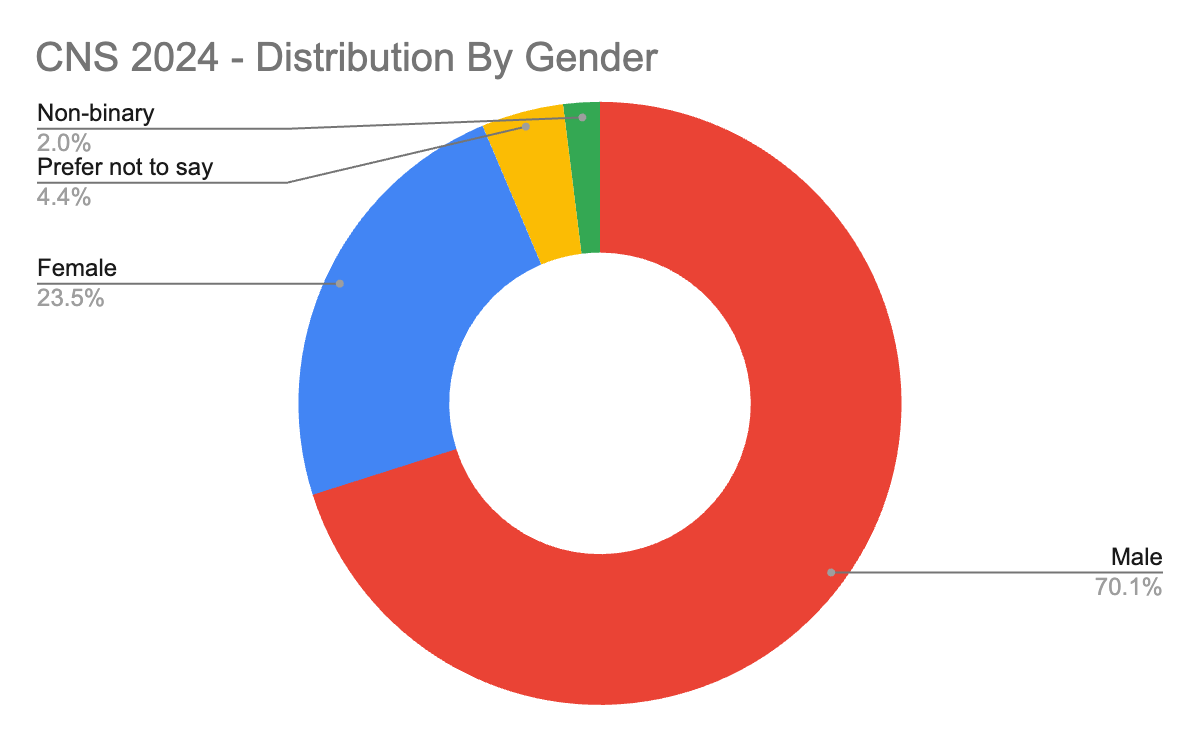
\includegraphics[width=0.9\textwidth]{images/cns2024-attendees-distribution-gender-1}
  %\caption{images/cns2024-attendees-distribution}%
  %\label{fig:images-cns2024-attendees-distribution}
\end{figure}
% to remove white background from the charts, use imagemagick:
% magick <input file> -fuzz 1%% -transparent White <output file>

\clearpage
\section*{CNS*2024 Natal: in charts}%
\vspace{-4ex}
\sectionauthor{}
\begin{figure}[ht]
  \centering
  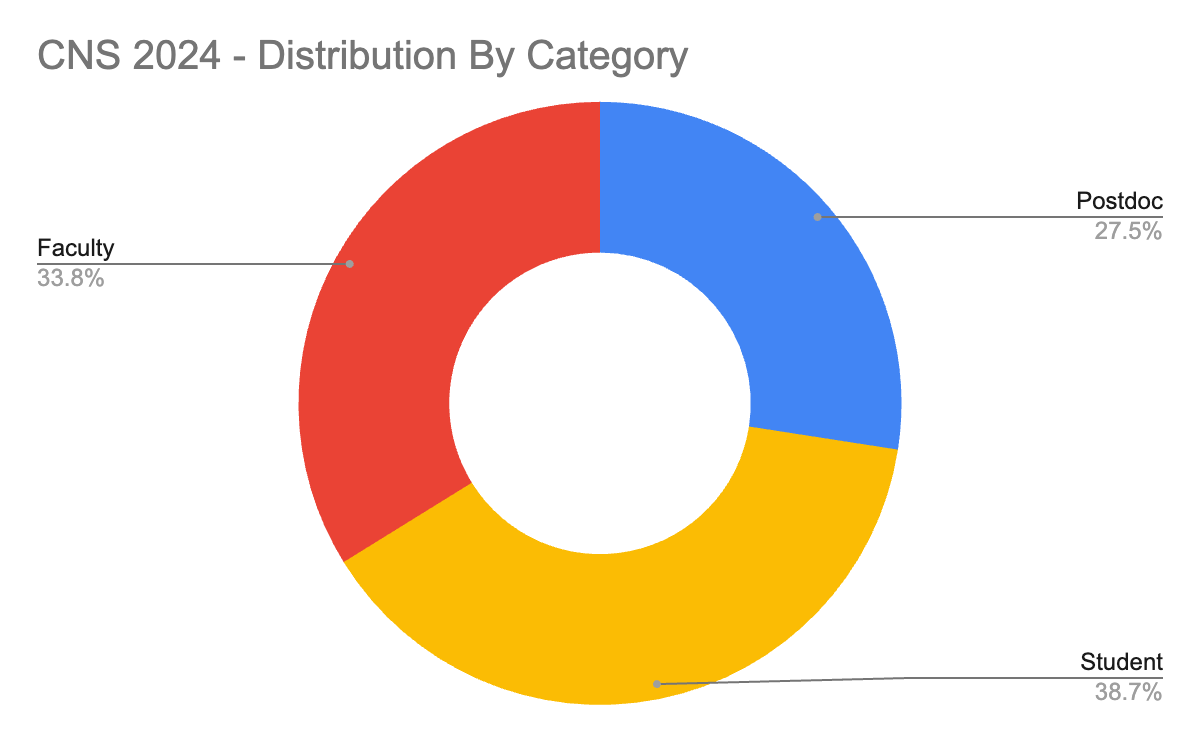
\includegraphics[width=0.9\textwidth]{images/cns2024-attendees-distribution-career-1}\\\vspace{3ex}
  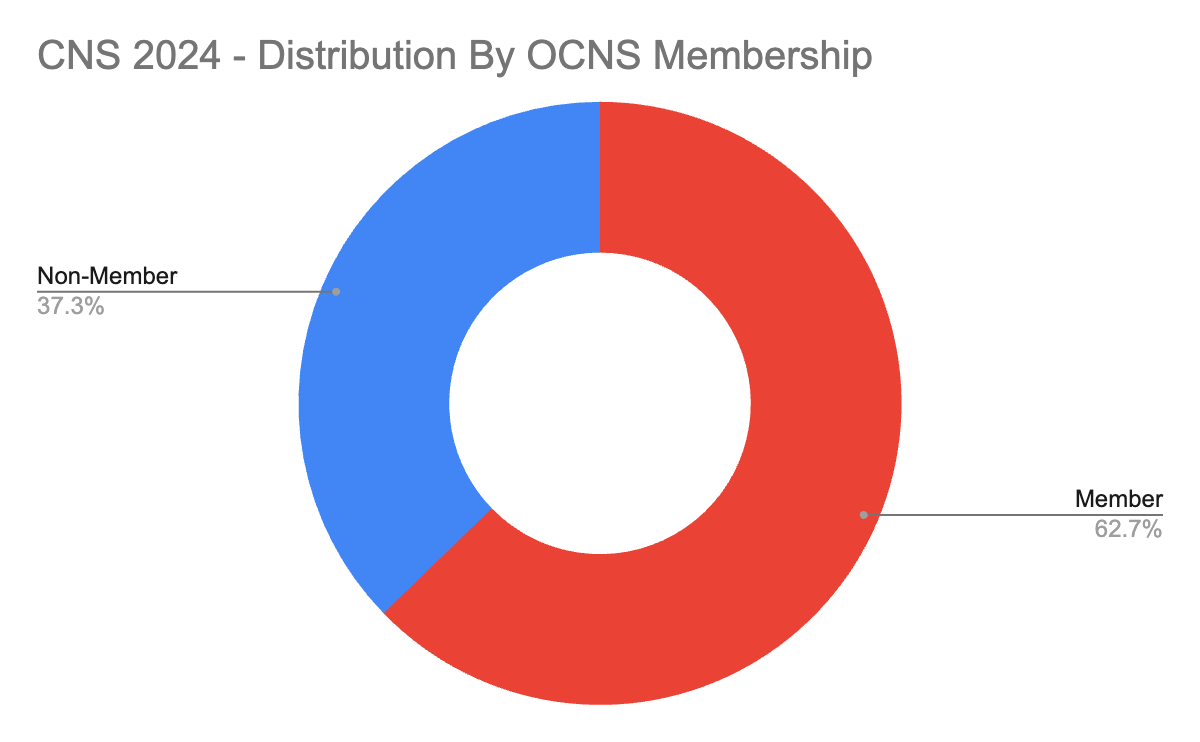
\includegraphics[width=0.9\textwidth]{images/cns2024-attendees-distribution-membership-1}\\
  %\caption{images/cns2024-attendees-distribution}%
  %\label{fig:images-cns2024-attendees-distribution}
\end{figure}

\clearpage
\section*{CNS*2024 Natal: Travel Awards}%
\sectionauthor{Travel Awards Chair:\ Michelle Moerel, Maastricht Centre for Systems Biology, Netherlands}
\begin{wrapfigure}{l}{0.2\textwidth}
  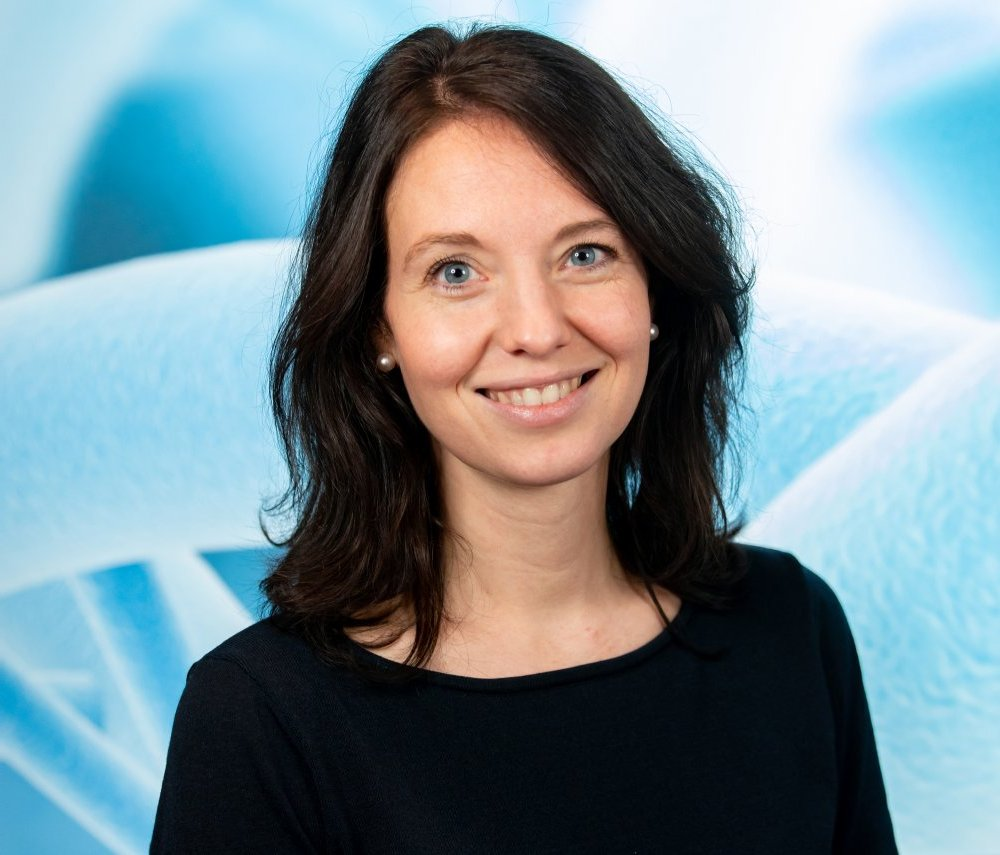
\includegraphics[width=0.2\textwidth]{images/Moerel}
\end{wrapfigure}

\noindent{}A limited number of merit based travel awards, given based on review of summaries by the program committee, are available to presenting students and postdocs who are OCNS members. Women and members of other historically marginalized communities in Science, Technology, Engineering, and Mathematics are particularly encouraged to apply.
Applications for travel grants are to be submitted during the abstract submission process at the annual OCNS conference.

This year's travel awards were competitive, with many more excellent applicants than available funds.
We were pleased to award 19 travel grants to participants from all over the world:

\begin{multicols}{2}
    \begin{itemize}
      \item Flavio Rusch (Brazil)
      \item Cecilia Jarne (Argentina)
      \item Paolo Protachevicz (Brazil)
      \item Fernando Fagundes Ferreira (Brazil)
      \item Pamela Alejandra Illescas Maldonado (Chile)
      \item Lavinia Mitiko Takarabe (Brazil)
      \item Forough Habibollahi Saatlou (Australia)
      \item Fabio Pioggio (Italy)
      \item Richard Gast (USA)
      \item Alexandra Chatzikalymniou (USA)
      \item Ankur Sinha (UK)
      \item Christopher Earl (USA)
      \item Anaelle De Worm (Belgium)
      \item Ferdinand Tixidre (France)
      \item Camille Mazzara (Italy)
      \item Lindsay Stolting (USA)
      \item Elnaz Nemati (Australia)
      \item Dirk Goldschmitt (UK)
      \item Eleonora Bernasconi (UK)
    \end{itemize}
\end{multicols}
\vspace{2ex}
\centerline{\rule{0.5\textwidth}{0.4pt}}
\vspace{4ex}
\noindent{}{\color{Blue}\textbf{\large Quotes from a few travel awardees:\\}}

\noindent{}\textbf{Flavio Rusch (Brazil)}
\begin{displayquote}
Attending CNS*2024 was an invaluable experience in my career as a physicist working in computational neuroscience. It provided me the opportunity to present my research to leading figures in the field, engage in discussions, and expand my network of collaborations. I am deeply grateful to OCNS for the travel award, as it made this opportunity possible.
\end{displayquote}

\vspace{2ex}
\noindent{}\textbf{Fabio Poggio (Italy)}
\begin{displayquote}
Receiving the travel award to attend CNS 2024 was a significant opportunity to engage with the latest advances in computational neuroscience and to exchange ideas with leading experts in the field. This experience has significantly enriched my research and professional growth, and I highly recommend it to anyone passionate about computational neuroscience.
\end{displayquote}
\clearpage
\noindent{}\textbf{Pamela Illescas (Chile)}
\begin{displayquote}
CNS 2024 in Natal was a wonderful experience to learn and share my doctoral thesis on networks with neuron-astrocyte interactions, which allowed
me to receive feedback from other researchers and opportunities for collaboration. This meeting was my first international computational neuroscience conference, and it was possible thanks to the CNS travel award. I am very grateful for this opportunity because it allows me to contribute to computational neuroscience in my country and internationally.
\end{displayquote}

\vspace{2ex}
\noindent{}\textbf{Cecilia Jarne, (Argentina)}
\begin{displayquote}
Attending CNS 2024 was an invaluable experience that allowed me to share our work on Hidden Markov Models (HMMs) software through the tutorial sessions offered at the conference. It also allowed me to present a poster on my ongoing research in predicting brain age, fostering meaningful discussions. I am very grateful for the travel award, which made this enriching experience possible.
\end{displayquote}




\clearpage
\section*{CNS*2024 Natal: Feedback form Summary}%
\sectionauthor{Registrations Chair:\ Tatiana Kameneva, Swinburne University of Technology, Australia}
\begin{wrapfigure}{l}{0.2\textwidth}
  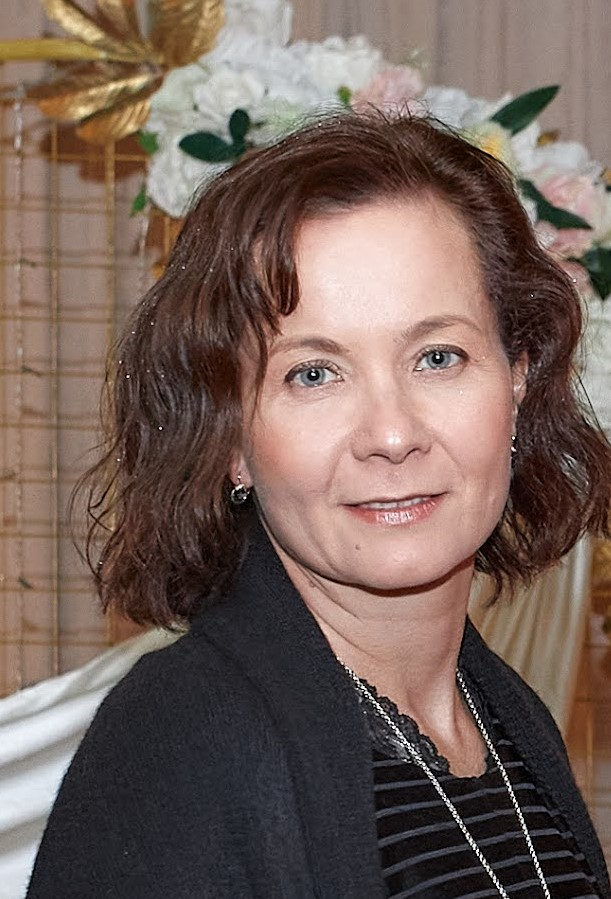
\includegraphics[width=0.2\textwidth]{images/Kameneva}
\end{wrapfigure}

We received 42 responses on the Participant Feedback Survey distributed at the end of CNS*2024.
Overall, the feedback has been positive. The data is presented in \cref{fig:cns2024-summary} above, with 5 being the highest rating.

Most people have enjoyed the venue: 71\% gave 4 or 5 rating in this category (\cref{fig:cns2024-summary} A).
Attendees commented highly on the quality of the keynote speakers: 55\% gave the highest (5) rating in this category (\cref{fig:cns2024-summary} B).
The common theme was a commendation to the local organizers for catering, efficiency, and airport pickup; while the AV, staff English proficiency, and the small space allocated for posters received mostly negative comments.

Tutorials had mixed reviews: 10\% of the attendees submitted the rating less than average satisfaction (1 or 2), while most people, 42\%, gave the rating 4 (\cref{fig:cns2024-summary} C). No comments were provided.

The attendance at the workshops varied.
Some workshops received very high praise; 80\% of people gave ratings 4 or 5, with comments such as \enquote{very interesting topics}, \enquote{amazing}, \enquote{excellent session} (\cref{fig:cns2024-summary} D).
While other workshops left attendees dissatisfied, with suggestions to reduce the number of parallel sessions to boost the attendance.

Overall, 79\% attendees enjoyed oral presentations and gave the ratings 4 or 5, while 21\% rated the presentation as satisfactory (3) or below (2), \cref{fig:cns2024-summary} E.
Positive comments included \enquote{OCNS is superb in supporting young scientist's careers}.
Suggestions for improvements included more talks on data-driven, deep learning-based approaches.
We thank everybody for their feedback that will be taken into account when organizing CNS*2025.

\begin{figure}[!h]
  \centering
  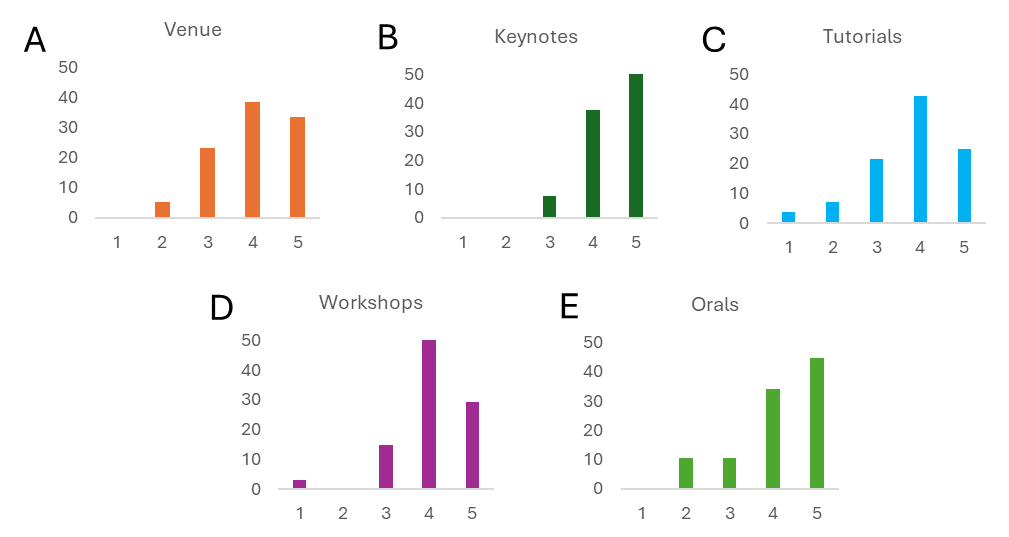
\includegraphics[width=\textwidth]{images/cns2024-feedback-form-summary}
  \caption{Summary of participant feedback, CNS*2024}%
  \label{fig:cns2024-summary}
\end{figure}


\clearpage

\section*{CNS*2025: Firenze (Florence), Italy: July 5--9, 2025}%
\sectionauthor{Michele Migliore\\Sergio Solinas}
\begin{figure}[ht]
  \centering
  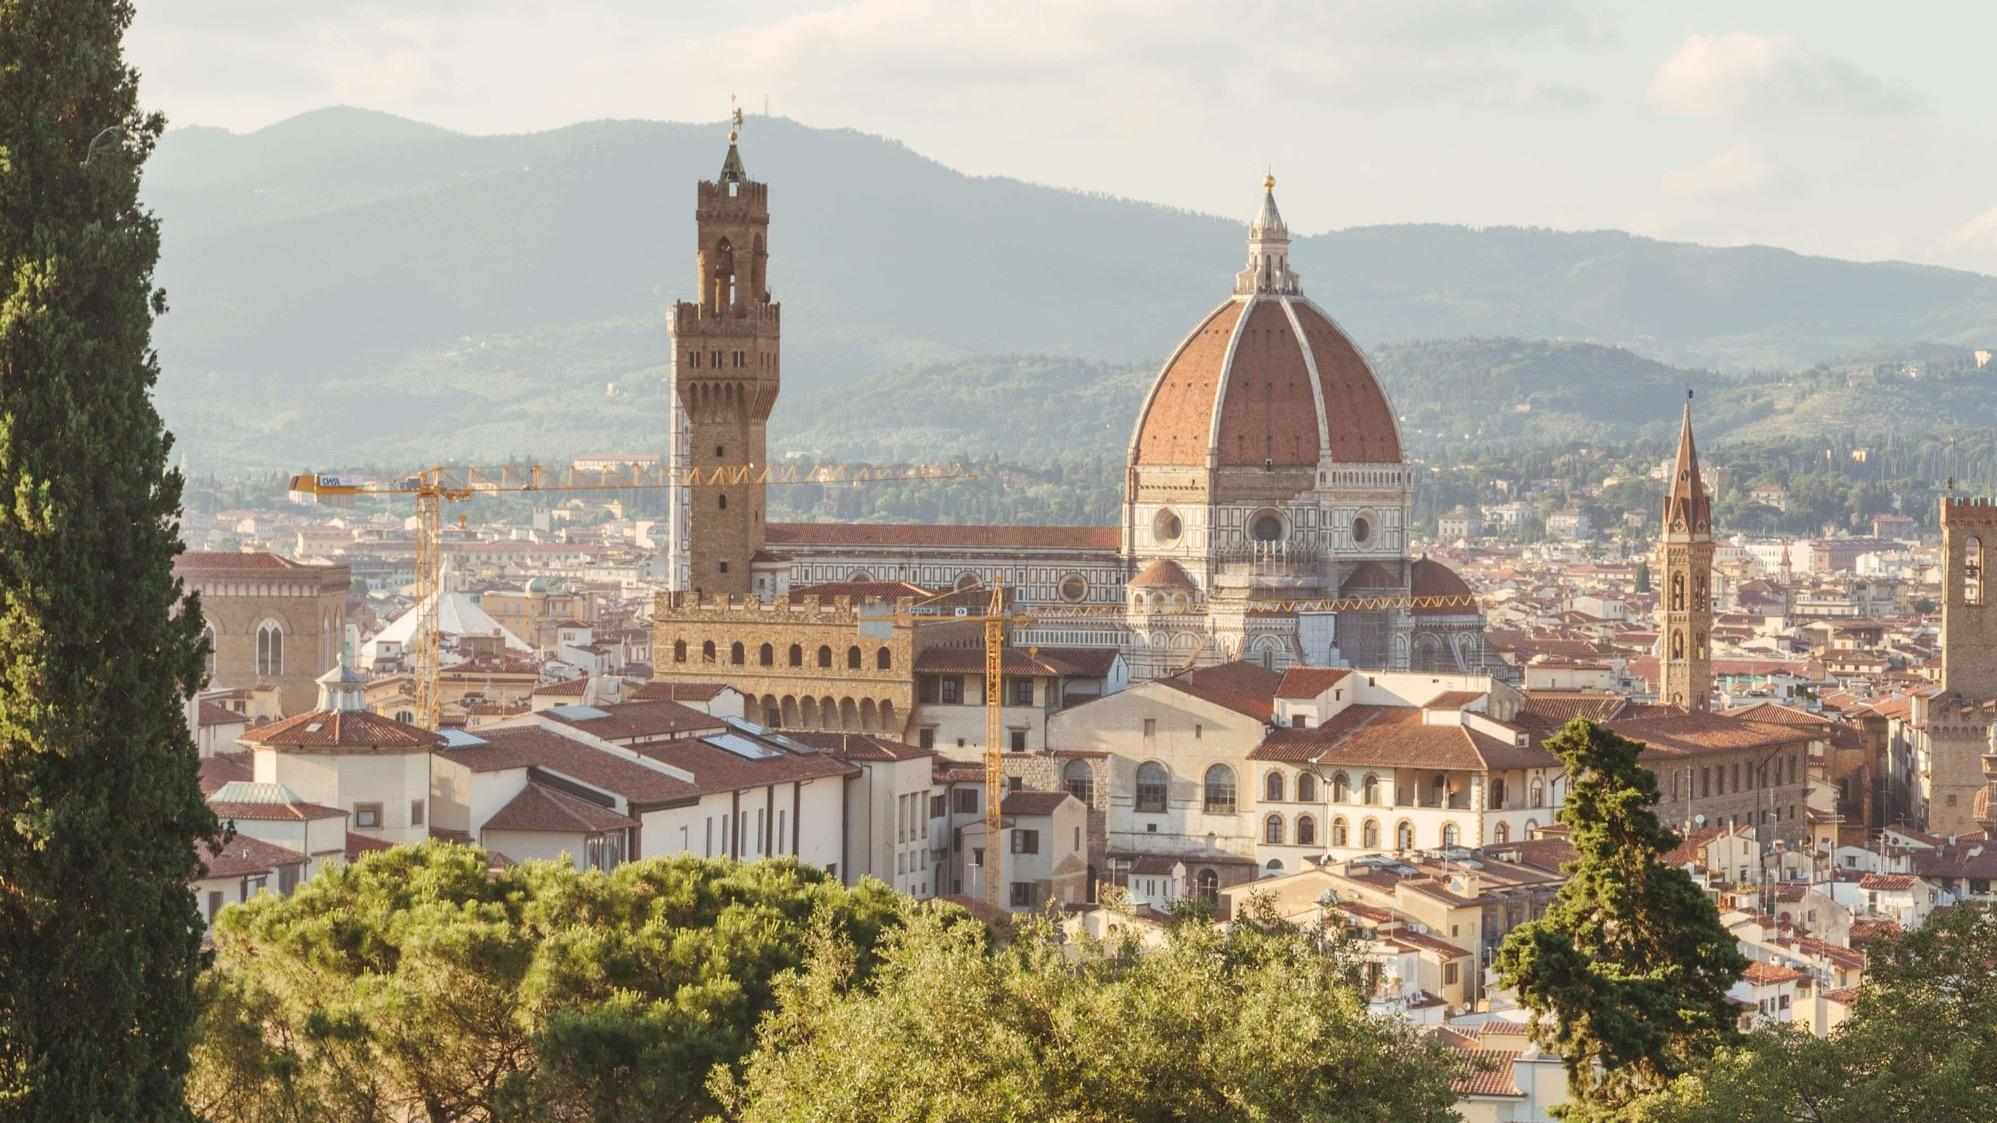
\includegraphics[width=\textwidth]{images/cns2025-florence}
\end{figure}

\begin{center}
\textcolor{Blue}{\textbf{\Large Florence: the cradle of the Renaissance}}
\end{center}

\vspace{1ex}
\centerline{\rule{0.5\textwidth}{0.4pt}}
\vspace{1ex}
\begin{center}
  \textcolor{Blue}{\textbf{\Large OCNS is excited to invite you to the\\\vspace{2ex}34th Annual Computational Neuroscience meeting\\\vspace{2ex}CNS*2025\\\vspace{2ex}{in}\\\vspace{2ex}Firenze (Florence), Italy from July 5--9, 2025.}}
\end{center}
\vspace{1ex}
\centerline{\rule{0.5\textwidth}{0.4pt}}
\vspace{2ex}
\begin{center}
\textcolor{Blue}{\textbf{\Large Please mark your calendars!}}
\end{center}

\clearpage
\section*{Note on CNS conference proceedings}%
\sectionauthor{Publications Chair:\ Ingo Bojak, University of Reading, UK}
Proceedings from the annual CNS conferences are published by the end of the year annually.
Links to proceedings from previous conferences are below:
\begin{multicols}{2}
    \begin{itemize}
      \item \href{https://link.springer.com/article/10.1007/s10827-024-00871-5}{CNS*2023 Leipzig} (\href{https://link.springer.com/article/10.1007/s10827-024-00872-4}{Introduction})
      \item \href{https://link.springer.com/article/10.1007/s10827-022-00841-9}{CNS*2022 Melbourne} (\href{https://link.springer.com/article/10.1007/s10827-022-00843-7}{Introduction})
    \end{itemize}
\end{multicols}

Proceedings from previous conferences are archived on the website here:

\begin{center}
\url{https://www.cnsorg.org/annual-meeting-publications}.
\end{center}

\centerline{\rule{0.5\textwidth}{0.4pt}}
\vspace{1ex}
{\color{Blue}\textbf{\large Note from the publisher, Springer Nature:}}

Each year, Journal of Computational Neuroscience publishes a supplement including abstracts from the CNS annual meeting.
In 2023, the CNS*22 abstracts supplement was published in January.
Changes in the supplement publishing process and our oversight in timely communicating the same to OCNS have regrettably delayed publication of the abstracts from CNS*23.
Proofs of this 2024 supplement are now being finalized.
Please accept our sincere apologies for the delay.
Springer Nature values the relationship between the Organization for Computational Neurosciences and Journal of Computational Neuroscience.
We look forward to the timely publication of future CNS supplements.


\clearpage
\section*{OCNS Board:\ New arrivals and members rotating off}%
\sectionauthor{\vspace{-4ex}}

The current board of directors consists of 23 elected and ex officio members.
According to the \href{https://www.cnsorg.org/ocns-bylaws-2011}{OCNS Bylaws}, \href{https://www.cnsorg.org/election-procedures}{elections} are held to replace three or four outgoing directors each year.
The board elects its officers.
The duties carried out by members of the board can be seen \href{https://www.cnsorg.org/quick-director-duties}{here}.

\textbf{Terms for a number of Board members were renewed this year:}
\begin{multicols}{2}
  \begin{itemize}
    \item Thomas Nowotny (President)
    \item Leonid Rubchinksy (Vice president)
    \item Gennady Cymbalyuk (Treasurer)
  \end{itemize}
\end{multicols}

\textbf{The following members have completed their terms and will rotate off at the end of 2024.}
\textbf{OCNS thanks them for their service:}
\begin{multicols}{2}
  \begin{itemize}
    \item Cengiz Gunay (Newsletter chair)
    \item Maurizio de Pitta (Tutorials chair)
    \item Christoph Metzner (Membership chair)
    \item Srikanth Ramaswamy (Workshops chair)
  \end{itemize}
\end{multicols}

\textbf{A number of new Board members were elected in the 2023 Elections, or have moved to new roles within the Board:}
\begin{multicols}{2}
  \begin{itemize}
    \item Shailesh Appukuttan (Publications chair)
    \item Michelle Moerel (Travel awards chair)
    \item Ankur Sinha (Newsletter chair)
    \item Robert McDougal (Webmaster)
    \item Rodrigo de Oliveira Pena (Membership chair)
    \item Anathanasia Papoutsi (Workshops chair)
    \item Kersink Lenk (Social media chair)
    \item Eirini Mavritsaki (EDI chair: new position)
  \end{itemize}
\end{multicols}

\section*{OCNS Board:\ Elections: Nominations are open!}%
\sectionauthor{\vspace{-4ex}}
The nomination period for self-nominations for the election of new members of the \href{}{OCNS Board of Directors} is now open.
New Directors will serve a three-year term from January 2025 through December 2027 and will initially fill the following roles:
\begin{multicols}{2}
  \begin{itemize}
    \item Registration Chair
    \item Sponsorship Chair
  \end{itemize}
\end{multicols}

New Directors will act as Deputy Chairs in their roles by shadowing the current Chairs for a year, and then will take over when the current Chairs finish their terms.
Candidates need to be current OCNS members and are required to have been OCNS members for at least a year or to attend an on-site CNS conference in the past.
More information about the new Directors' election can be found at:

\begin{center}
\url{https://www.cnsorg.org/election-procedures}
\end{center}


We strongly encourage OCNS members to consider self-nomination for these elections.

%\begin{tcolorbox}[colback=CornflowerBlue, colframe=black, width=\textwidth, boxrule=0.1mm, leftrule=0.1mm, rightrule=0mm]
\begin{tcolorbox}[colback=CornflowerBlue, colframe=black, width=\textwidth, boxrule=0.1mm]
\textbf{OCNS is committed to have a wide diversity among its Directors---across research areas, gender, abilities, career experiences, geographic locations, and personal backgrounds.
This is possible only if a broad range of members apply.
This year we are looking to appoint at least one student/postdoc Board Member.
The OCNS strives to be a diverse group and encourages a balanced and inclusive representation of women in leadership positions within the organization.}
\end{tcolorbox}

Please contact our EDI Chair Eirini Mavritsaki (\href{mailto:eirini.mavritsaki@bcu.ac.uk}{eirini.mavritsaki@bcu.ac.uk}) if you wish to have a short informational meeting about joining the board.

To apply, please use the form:

\begin{center}
\url{https://www.cnsorg.org/board-nomination-2024}
\end{center}

The deadline for application is \underline{October 16, 2024}.

\clearpage
\section*{OCNS Membership}%
\sectionauthor{\vspace{-4ex}}

The OCNS membership consists of:
\begin{table}[!h]
  \centering
  \begin{tabularx}{0.7\textwidth}{X|ccccc}
    \textbf{Member type}& \textbf{2024} & \textbf{2023} & \textbf{2022} & \textbf{2021} & \textbf{2020} \\
    \toprule{}
    Student & \textbf{139} &  185 & 182 & 212 & 266 \\
    Post-doc/not-for-profit employee & \textbf{93} & 135 & 118 & 141 & 155 \\
    Faculty/for-profit emplyoee & \textbf{179} & 215 & 209 & 217 & 189 \\
    \midrule{}
    Total & \textbf{401} & 535 & 509 & 570 & 610 \\
  \end{tabularx}
\end{table}

Membership type definitions:
\begin{itemize}
  \item \textbf{Student:} Anybody studying toward an undergraduate or graduate degree.
  \item \textbf{Postdoc/not-for-profit employee:} Anybody who is employed as a postdoctoral scholar or postdoctoral fellow, and anybody who is employed in a university lab or non-industry research institute as a technician or research assistant not seeking a degree.
  \item \textbf{Faculty/for-profit employee:} Anybody who is employed as faculty, laboratory head, independent researcher, or in an equivalent position, and anybody who is employed in industry or for-profit institutions
  \item Retired persons should apply for or remain in their pre-retirement category.
\end{itemize}

\section*{Membership Benefits}%
\sectionauthor{\vspace{-4ex}}

OCNS members enjoy a number of rights and \href{https://www.cnsorg.org/member-benefits}{benefits}:
\begin{multicols}{2}
  \begin{itemize}
    \item Reduced conference registration fees
    \item Eligibility for travel awards
    \item Nomination and voting rights for OCNS director elections
    \item Special Interest Groups (SIGs)
    \item Computational neuroscience schools
    \item Submission of extra abstract to the conference
    \item Free access to Springer encyclopedia
    \item Reduced journal subscription fees
    \item Book discounts
  \end{itemize}
\end{multicols}

\section*{Membership Renewal}%
\sectionauthor{\vspace{-4ex}}

To \textbf{renew} your OCNS membership, please login at \href{www.cnsorg.org}{www.cnsorg.org} to pay your OCNS dues.
Please note that renewing with a multiple year membership will reduce your costs:

\begin{table}[!h]
  \centering
  \begin{tabularx}{0.7\textwidth}{X|ccc}
    \textbf{Member type}& \textbf{One year} & \textbf{Two years} & \textbf{Three years} \\
    \toprule{}
    Student & 10 USD & 15 USD & 20 USD \\
    Post-doc/not-for-profit employee & 20 USD & 30 USD & 40 USD \\
    Faculty/for-profit emplyoee& 50 USD & 75 USD & 100 USD \\
  \end{tabularx}
\end{table}

Please contact the Membership Chair at \href{mailto:membership@cnsorg.org}{membership@cnsorg.org} before you pay your dues if:
\begin{itemize}
  \item You are uncertain which category is appropriate for you.
  \item Your employment status has changed.
\item \emph{If you believe that special circumstances prohibit you from paying the full dues.}
\end{itemize}


\clearpage
\section*{Initiatives: Software Working Group}%
\sectionauthor{Marcel Stimberg, Sorbonne Universite, Paris, France\\
Ankur Sinha, University College London, UK}

The Software Working Group aims to increase awareness and knowledge of the various software tools that we use to carry out our research.
The group is an open community group that everyone is welcome to join.
It is shared between the OCNS and the \href{https://incf.org}{International Neuroinformatics Co-ordinating Facility (INCF)}, of which OCNS is a member organization.

In the past year, the group has continued to host sessions on different neuroscience software.
Recordings from these sessions can be found on the \href{https://www.youtube.com/@IncfOrg_INCF/videos}{INCF YouTube channel}, and also on the \href{https://training.incf.org/course/incfocns-working-group-computational-neuroscience-software}{INCF Training Space}.
Working group announcements are published on our \href{https://ocns.github.io/SoftwareWG/}{website}.

If there are software tools/standards that you think are useful for the community to know and learn about, please contact either of the working group co-chairs to let us know (\href{mailto:marcel.stimberg@sorbonne-universite.fr}{marcel.stimberg@sorbonne-universite.fr}, \href{mailto:ankur.sinha@ucl.ac.uk}{ankur.sinha@ucl.ac.uk}).
We will reach out to the developers of the software to organize a session on it.

The working group also sets up task forces to work on specific projects.
Currently, a task force is working on developing a simple web based tool to help community members decide what simulation tool they should use.
A working title for this tool is \href{https://github.com/OCNS/simselect/issues}{Simselect}. 
If you would like to get involved in this task force, please let us know.

\section*{Initiatives: Mentoring Program Updates}%
\sectionauthor{EDI Chair: Eirini Mavristaki, Birmingham City University, UK}
\begin{wrapfigure}{l}{0.2\textwidth}
  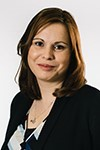
\includegraphics[width=0.2\textwidth]{images/Mavritsaki}
\end{wrapfigure}

\lipsum[1-2]

\clearpage
\section*{Messages from our Sponsors}%
\sectionauthor{Short messages from OCNS sponsors}
\subsection*{Metacell}%
\begin{displayquote}
  Thank you to OCNS for hosting an excellent annual meeting, and to everyone who connected with MetaCell, attended our presentation and joined our event.
  It was great catching up with friends and partners in Natal, and we were proud sponsors of the meeting!

  If you're interested in new ways to standardize, visualize, share, and build your computational models, please visit \url{metacell.us} and get in touch with our team.
\end{displayquote}

\clearpage
\section*{INCF Updates}%
\sectionauthor{Helena/Matthew}
\lipsum[1-3]

\clearpage
% break into separate file, since we expect this to be along section
\section*{OCNS:\ Member Updates: Scientific Items}%
\sectionauthor{Updates of scientific interest from OCNS members}

\noindent{}The name of the OCNS member that submitted the entry is highlighted in \textbf{bold}.

\nocite{*}
\printbibliography[heading=none]

\clearpage
% break into separate file, since we expect this to be along section
\section*{OCNS: Member Updates: Community Development}%
\sectionauthor{Updates related to community development from OCNS members}

\begin{itemize}
    \item \textbf{The Capo Caccia Worskhops toward Neuromorphic Intelligence}

        Submitted by: Mihai A Petrovici

        \url{https://capocaccia.cc/en/event/ccnw24/landing-page/}

        The goal of the CCNW workshops is to promote the neuromorphic approach to designing technologies, establish an international community, and to encourage collaboration amongst small groups, in order to achieve the kind of technical advances which could only otherwise happen in well-funded industrial labs.

        The CCNW has an open format, whose intention is to encourage creativity and exploration of ideas and projects in a relaxed and intellectually open environment. Although there is a skeleton program that sets a default route through the two weeks, ad hoc deviations from or elaborations of this basic program are encouraged. Discussion groups and projects arise dynamically. There are no formal lectures. Instead, the morning consist of two 1.5 hr discussion sessions in which a few discussants will make short contributions to the topics in order to ignite more general interaction. Although the sessions of the skeleton program have assigned moderators and discussants, these persons should also be seen as defaults. Whiteboards and overhead tablets are available for drawings. Formal presentations with prepared media (such as Powerpoint slides) are strictly forbidden. The daily program includes a late afternoon sports break, and happy hour.


    \item \textbf{The Lu.i educational neurons}

        Submitted by: Mihai A Petrovici

        \url{https://physiologie.unibe.ch/~petrovici/group/lui.aspx}

        With an increasing presence of science throughout all parts of society, there is a rising expectation for researchers to effectively communicate their work and, equally, for teachers to discuss contemporary findings in their classrooms. While the community can resort to an established set of teaching aids for the fundamental concepts of most natural sciences, there is a need for similarly illustrative experiments and demonstrators in neuroscience. We therefore introduce Lu.i: a parametrizable electronic implementation of the leaky-integrate-and-fire neuron model in an engaging form factor. These palm-sized neurons can be used to visualize and experience the dynamics of individual cells and small spiking neural networks. When stimulated with real or simulated sensory input, Lu.i demonstrates brain-inspired information processing in the hands of a student. As such, it is actively used at workshops, in classrooms, and for science communication. As a versatile tool for teaching and outreach, Lu.i nurtures the comprehension of neuroscience research and neuromorphic engineering among future generations of scientists and in the general public.

    \item \textbf{Neuroscience Gateway (NSG)}

        Submitted by: Amitava Majumdar

        \url{https://www.nsgportal.org}

        NSG project provides free and open access to supercomputing resources. NSG enables modeling, simulation and data processing (e.g. EEG, MEG, fMRI etc.) research in neuroscience by lowering the administrative and technical barriers that currently make it difficult for investigators to use large scale computing resources. It provides access to popular neuroscience tools, pipelines, data processing software and libraries.


\end{itemize}
\newpage
\begin{itemize}
    \item \textbf{Advanced Scientific Programming in Python Summer School}

        Submitted by: Anathanasia \enquote{Nassi} Papoutsi

        \url{https://aspp.school}

        The Institute of Molecular Biology and Biotechnology of the Foundation for Research and Technology Hellas (IMBB-FORTH) at Heraklion, Crete, Greece hosted the 16th Advanced Scientific Programming in Python Summer School from August 26th to August 31st, 2024. The Summer School, kindly funded by Tubingen AI Center, was attended by 30 participants from all over the world. The interactive lectures, pair programming sessions, and coding tournaments made for an unforgettable experience. A huge thanks to our amazing participants, faculty, and organizers for bringing so much energy and enthusiasm!

\end{itemize}


\clearpage
\vspace*{\fill}
\begin{center}
  \begin{minipage}{\textwidth}
    \begin{center}
      Copyright \textcopyright{} OCNS 2024.

      The OCNS newsletter is distributed under the \href{https://creativecommons.org/licenses/by-nc-nd/4.0/}{CC By-NC-ND} license.

      Please contact the newsletter chair at \href{mailto:newsletter@cnsorg.org}{newsletter@cnsorg.org} for any clarifications, comments, and remarks.
    \end{center}
  \end{minipage}
\end{center}
\vfill
\clearpage
\end{document}

